% Options for packages loaded elsewhere
\PassOptionsToPackage{unicode}{hyperref}
\PassOptionsToPackage{hyphens}{url}
%
\documentclass[
]{article}
\usepackage{lmodern}
\usepackage{amssymb,amsmath}
\usepackage{ifxetex,ifluatex}
\ifnum 0\ifxetex 1\fi\ifluatex 1\fi=0 % if pdftex
  \usepackage[T1]{fontenc}
  \usepackage[utf8]{inputenc}
  \usepackage{textcomp} % provide euro and other symbols
\else % if luatex or xetex
  \usepackage{unicode-math}
  \defaultfontfeatures{Scale=MatchLowercase}
  \defaultfontfeatures[\rmfamily]{Ligatures=TeX,Scale=1}
\fi
% Use upquote if available, for straight quotes in verbatim environments
\IfFileExists{upquote.sty}{\usepackage{upquote}}{}
\IfFileExists{microtype.sty}{% use microtype if available
  \usepackage[]{microtype}
  \UseMicrotypeSet[protrusion]{basicmath} % disable protrusion for tt fonts
}{}
\makeatletter
\@ifundefined{KOMAClassName}{% if non-KOMA class
  \IfFileExists{parskip.sty}{%
    \usepackage{parskip}
  }{% else
    \setlength{\parindent}{0pt}
    \setlength{\parskip}{6pt plus 2pt minus 1pt}}
}{% if KOMA class
  \KOMAoptions{parskip=half}}
\makeatother
\usepackage{xcolor}
\IfFileExists{xurl.sty}{\usepackage{xurl}}{} % add URL line breaks if available
\IfFileExists{bookmark.sty}{\usepackage{bookmark}}{\usepackage{hyperref}}
\hypersetup{
  pdftitle={Some Demographic Changes from 2010},
  pdfauthor={Paul Collins},
  hidelinks,
  pdfcreator={LaTeX via pandoc}}
\urlstyle{same} % disable monospaced font for URLs
\usepackage[margin=1in]{geometry}
\usepackage{graphicx,grffile}
\makeatletter
\def\maxwidth{\ifdim\Gin@nat@width>\linewidth\linewidth\else\Gin@nat@width\fi}
\def\maxheight{\ifdim\Gin@nat@height>\textheight\textheight\else\Gin@nat@height\fi}
\makeatother
% Scale images if necessary, so that they will not overflow the page
% margins by default, and it is still possible to overwrite the defaults
% using explicit options in \includegraphics[width, height, ...]{}
\setkeys{Gin}{width=\maxwidth,height=\maxheight,keepaspectratio}
% Set default figure placement to htbp
\makeatletter
\def\fps@figure{htbp}
\makeatother
\setlength{\emergencystretch}{3em} % prevent overfull lines
\providecommand{\tightlist}{%
  \setlength{\itemsep}{0pt}\setlength{\parskip}{0pt}}
\setcounter{secnumdepth}{-\maxdimen} % remove section numbering
\usepackage{booktabs}
\usepackage{longtable}
\usepackage{array}
\usepackage{multirow}
\usepackage{wrapfig}
\usepackage{float}
\usepackage{colortbl}
\usepackage{pdflscape}
\usepackage{tabu}
\usepackage{threeparttable}
\usepackage{threeparttablex}
\usepackage[normalem]{ulem}
\usepackage{makecell}
\usepackage{xcolor}

\title{Some Demographic Changes from 2010}
\author{Paul Collins}
\date{06/03/2020}

\begin{document}
\maketitle

\hypertarget{this-is-a-pdf-document-of-the-county-wide-changes-from-the-2010-census-to-the-2018-american-communities-survey}{%
\section{This is a PDF Document of The County Wide Changes from the 2010
Census to the 2018 American Communities
Survey}\label{this-is-a-pdf-document-of-the-county-wide-changes-from-the-2010-census-to-the-2018-american-communities-survey}}

\hypertarget{it-is-to-show-what-pdfs-output-look-like-from-r}{%
\subsubsection{It is to show what PDF's Output Look Like from
R}\label{it-is-to-show-what-pdfs-output-look-like-from-r}}

Here's some words

\begin{verbatim}
##  [1] "Location"                                           
##  [2] "2010 Census: White"                                 
##  [3] "2010 Census: African American"                      
##  [4] "2010 Census: American Indian or Alaskan Native"     
##  [5] "2010 Census: Asian"                                 
##  [6] "2010 Census: Native Hawaiian or Pacific Islander"   
##  [7] "2010 Census: Two or More Races"                     
##  [8] "2018 ACS: White"                                    
##  [9] "2018 ACS: African American"                         
## [10] "2018 ACS: American Indian or Alaskan Native"        
## [11] "2018 ACS: Asian"                                    
## [12] "2018 ACS: Native Hawaiian or Pacific Islander"      
## [13] "2018 ACS: Two or More Races"                        
## [14] "Total Change: White"                                
## [15] "Total Change: African American"                     
## [16] "Total Change: American Indian or Alaska Native"     
## [17] "Total Change: Asian"                                
## [18] "Total Change: Native Hawaiian or Pacific Islander"  
## [19] "Total Change: Two or more Races"                    
## [20] "Percent Change: White"                              
## [21] "Percent Change: African American"                   
## [22] "Percent Change: American Indian or Alaska Native"   
## [23] "Percent Change: Asian"                              
## [24] "Percent Change: Native Hawaiian or Pacific Islander"
## [25] "Percent Change: Two or more Races"
\end{verbatim}

\hypertarget{heres-a-plot}{%
\subsection{Heres a plot}\label{heres-a-plot}}

This shows how plots look in the PDF, ignore the scaling as I ran out of
time doing this, but its an easy fix.

\includegraphics{changes_files/figure-latex/pressure-1.pdf}

\hypertarget{hawkins-county-age-group-changes-plot}{%
\subsection{Hawkins County Age Group Changes
Plot}\label{hawkins-county-age-group-changes-plot}}

Population is getting a lot older

\includegraphics{changes_files/figure-latex/hawkins county age group plot-1.pdf}

\hypertarget{add-extra-images-from-other-places-in}{%
\subsection{Add extra Images from Other Places
in}\label{add-extra-images-from-other-places-in}}

\begin{figure}
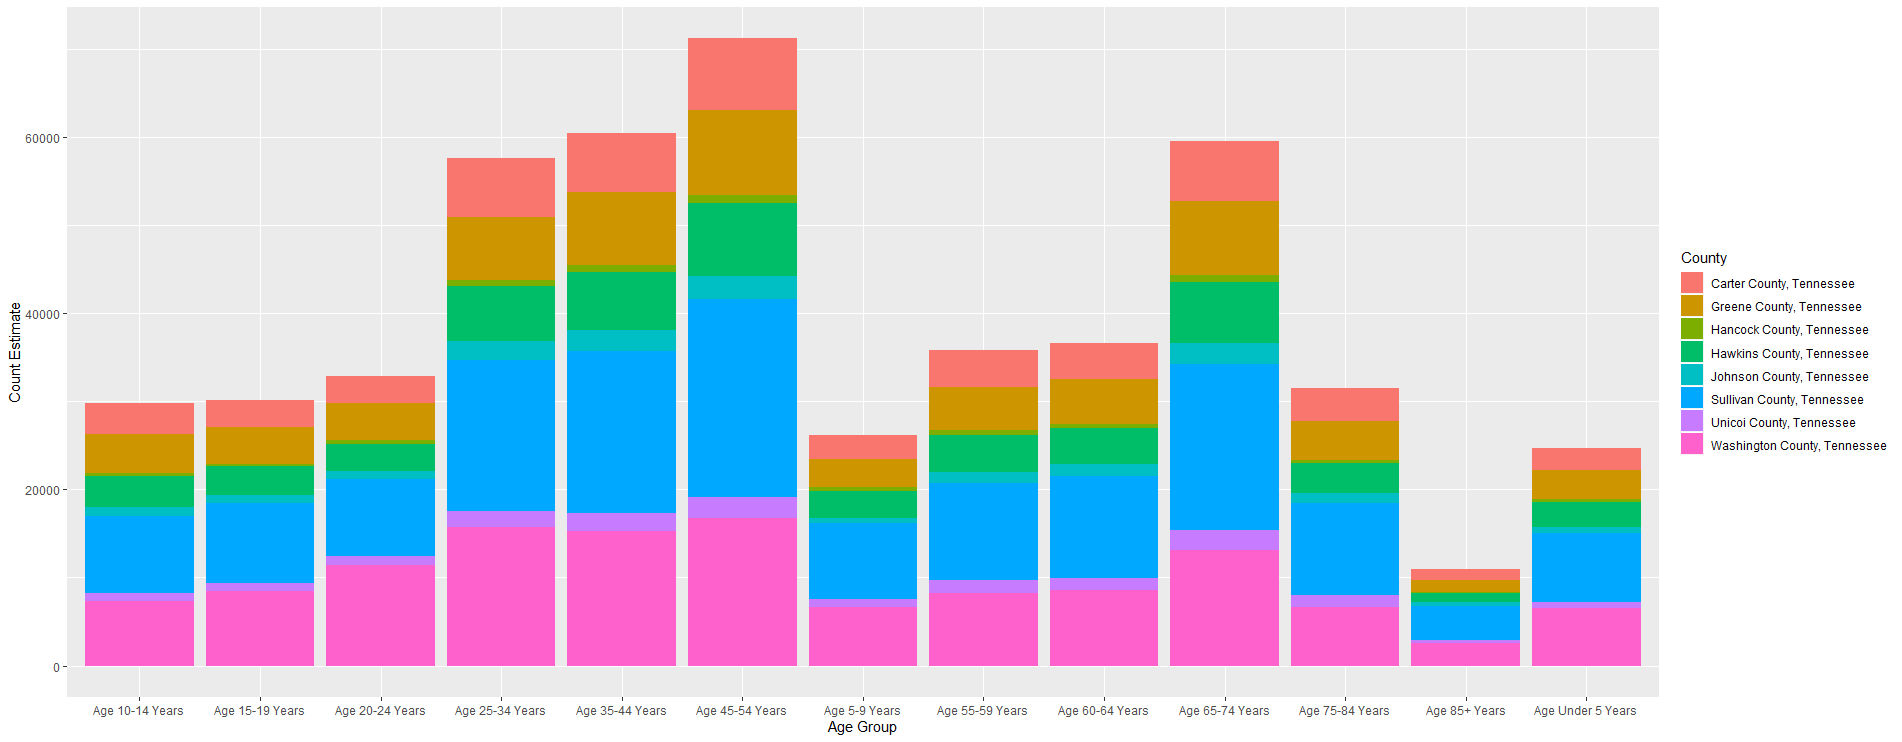
\includegraphics[width=1\linewidth]{age_group_plots} \caption{Age Group by County}\label{fig:age group by county}
\end{figure}

\hypertarget{map}{%
\subsection{Map}\label{map}}

Here is what a static image of those maps looks like in markdown PDF

\begin{figure}
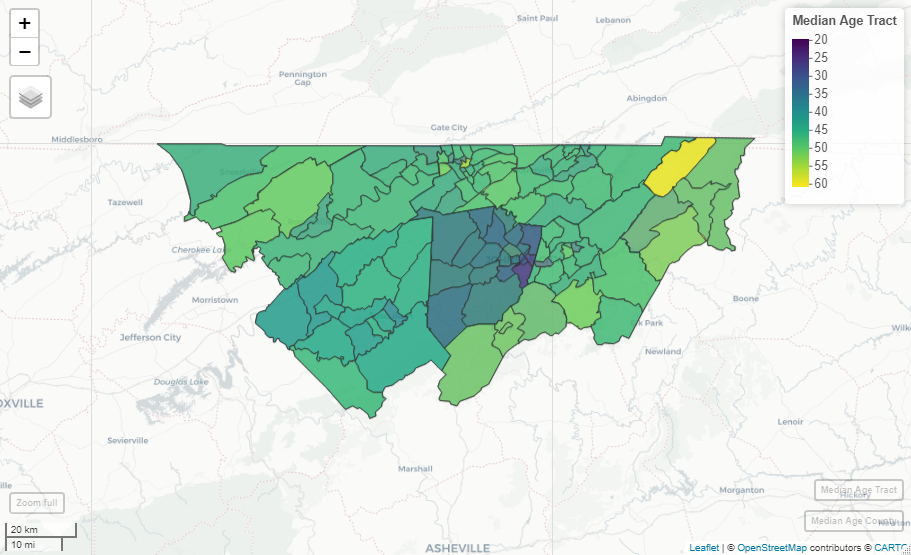
\includegraphics[width=1\linewidth]{median_age_mape} \caption{Median Age by Census Tract}\label{fig:static map}
\end{figure}

\hypertarget{population-change-table}{%
\subsubsection{Population Change Table}\label{population-change-table}}

\begin{table}

\caption{\label{tab:population table}Population Changes}
\centering
\resizebox{\linewidth}{!}{
\begin{tabular}[t]{lrrrr}
\toprule
Location & Census 2010 Population & ACS 2018 Estimate & Population Change & Pop. Percent Change\\
\midrule
\rowcolor{gray!6}  United States & 308745538 & 327167434 & 18421896 & 5.97\\
Tennessee & 6346105 & 6770010 & 423905 & 6.68\\
\rowcolor{gray!6}  Carter County, Tennessee & 57424 & 56351 & -1073 & -1.87\\
Greene County, Tennessee & 68831 & 69087 & 256 & 0.37\\
\rowcolor{gray!6}  Johnson County, Tennessee & 18244 & 17778 & -466 & -2.55\\
\addlinespace
Hancock County, Tennessee & 6819 & 6549 & -270 & -3.96\\
\rowcolor{gray!6}  Hawkins County, Tennessee & 56833 & 56530 & -303 & -0.53\\
Sullivan County, Tennessee & 156823 & 157668 & 845 & 0.54\\
\rowcolor{gray!6}  Washington County, Tennessee & 122979 & 128607 & 5628 & 4.58\\
Unicoi County, Tennessee & 18313 & 17761 & -552 & -3.01\\
\bottomrule
\end{tabular}}
\end{table}

\begin{table}[H]
\centering
\resizebox{\linewidth}{!}{
\begin{tabular}{lrrll}
\toprule
Location & Census 2010 Population & ACS 2018 Estimate & Population Change & Pop. Percent Change\\
\midrule
\rowcolor{gray!6}  United States & 308745538 & 327167434 & \textcolor{green}{18421896} & \textcolor{green}{5.97}\\
Tennessee & 6346105 & 6770010 & \textcolor{green}{423905} & \textcolor{green}{6.68}\\
\rowcolor{gray!6}  Carter County, Tennessee & 57424 & 56351 & \textcolor{red}{-1073} & \textcolor{red}{-1.87}\\
Greene County, Tennessee & 68831 & 69087 & \textcolor{green}{256} & \textcolor{green}{0.37}\\
\rowcolor{gray!6}  Johnson County, Tennessee & 18244 & 17778 & \textcolor{red}{-466} & \textcolor{red}{-2.55}\\
\addlinespace
Hancock County, Tennessee & 6819 & 6549 & \textcolor{red}{-270} & \textcolor{red}{-3.96}\\
\rowcolor{gray!6}  Hawkins County, Tennessee & 56833 & 56530 & \textcolor{red}{-303} & \textcolor{red}{-0.53}\\
Sullivan County, Tennessee & 156823 & 157668 & \textcolor{green}{845} & \textcolor{green}{0.54}\\
\rowcolor{gray!6}  Washington County, Tennessee & 122979 & 128607 & \textcolor{green}{5628} & \textcolor{green}{4.58}\\
Unicoi County, Tennessee & 18313 & 17761 & \textcolor{red}{-552} & \textcolor{red}{-3.01}\\
\bottomrule
\end{tabular}}
\end{table}

\hypertarget{age-group-table}{%
\subsubsection{Age Group Table}\label{age-group-table}}

\begin{table}[H]

\caption{\label{tab:age group table}Age Group Changes}
\centering
\resizebox{\linewidth}{!}{
\begin{tabular}[t]{l|r|r|r|r|r|r|r|r|r|r|r|r}
\hline
Location & 2010 Census: Age 0-5 Years & 2010 Census: Age over 65 Years & 2010 Census: Median Age & 2018 ACS: Age 0-5 Years & 2018 ACS: Age over 65 Years & 2018 ACS: Median Age & Total Change: Age 0-5 Years & Total Change: Age over 65 Years & Median Age Change & Percent Change: Age 0-5 Years & Percent Change: Age over 65 Years & Median Age Percent Change\\
\hline
United States & 20201362 & 40267984 & 37 & 19810275 & 52431193 & 38 & -391087 & 12163209 & 1 & -1.94 & 30.21 & 2.70\\
\hline
Tennessee & 407813 & 853462 & 38 & 406574 & 1109697 & 39 & -1239 & 256235 & 1 & -0.30 & 30.02 & 2.63\\
\hline
Carter County, Tennessee & 3041 & 9818 & 42 & 2534 & 12364 & 46 & -507 & 2546 & 4 & -16.67 & 25.93 & 9.52\\
\hline
Greene County, Tennessee & 3672 & 12006 & 43 & 3353 & 14918 & 45 & -319 & 2912 & 2 & -8.69 & 24.25 & 4.65\\
\hline
Johnson County, Tennessee & 901 & 3228 & 43 & 747 & 4056 & 46 & -154 & 828 & 3 & -17.09 & 25.65 & 6.98\\
\hline
Hancock County, Tennessee & 385 & 1159 & 43 & 352 & 1396 & 45 & -33 & 237 & 2 & -8.57 & 20.45 & 4.65\\
\hline
Hawkins County, Tennessee & 3161 & 9367 & 42 & 2709 & 11944 & 46 & -452 & 2577 & 4 & -14.30 & 27.51 & 9.52\\
\hline
Sullivan County, Tennessee & 8232 & 29215 & 44 & 7622 & 34529 & 45 & -610 & 5314 & 1 & -7.41 & 18.19 & 2.27\\
\hline
Washington County, Tennessee & 6666 & 18761 & 39 & 6398 & 23564 & 40 & -268 & 4803 & 1 & -4.02 & 25.60 & 2.56\\
\hline
Unicoi County, Tennessee & 933 & 3601 & 45 & 799 & 4123 & 47 & -134 & 522 & 2 & -14.36 & 14.50 & 4.44\\
\hline
\end{tabular}}
\end{table}

\hypertarget{racial-group-table}{%
\subsubsection{Racial Group Table}\label{racial-group-table}}

\begin{table}[H]
\centering
\resizebox{\linewidth}{!}{
\begin{tabular}{lrrrrrrrrrrrrrrrrrrlrrrrr}
\toprule
Location & 2010 Census: White & 2010 Census: African American & 2010 Census: American Indian or Alaskan Native & 2010 Census: Asian & 2010 Census: Native Hawaiian or Pacific Islander & 2010 Census: Two or More Races & 2018 ACS: White & 2018 ACS: African American & 2018 ACS: American Indian or Alaskan Native & 2018 ACS: Asian & 2018 ACS: Native Hawaiian or Pacific Islander & 2018 ACS: Two or More Races & Total Change: White & Total Change: African American & Total Change: American Indian or Alaska Native & Total Change: Asian & Total Change: Native Hawaiian or Pacific Islander & Total Change: Two or more Races & Percent Change: White & Percent Change: African American & Percent Change: American Indian or Alaska Native & Percent Change: Asian & Percent Change: Native Hawaiian or Pacific Islander & Percent Change: Two or more Races\\
\midrule
\rowcolor{gray!6}  United States & 248067530 & 43213173 & 6138482 & 17676507 & 1332494 & 6984195 & 258080572 & 47841851 & 6873732 & 22613335 & 1592094 & 8946480 & 10013042 & 4628678 & 735250 & 4936828 & 259600 & 1962285 & \textcolor{green}{4.04} & 10.71 & 11.98 & 27.93 & 19.48 & 28.10\\
Tennessee & 5144638 & 1117173 & 62526 & 115280 & 9359 & 96205 & 5437545 & 1227260 & 75025 & 159793 & 11880 & 132259 & 292907 & 110087 & 12499 & 44513 & 2521 & 36054 & \textcolor{green}{5.69} & 9.85 & 19.99 & 38.61 & 26.94 & 37.48\\
\rowcolor{gray!6}  Carter County, Tennessee & 56312 & 1041 & 418 & 270 & 44 & 624 & 55010 & 1239 & 516 & 328 & 41 & 745 & -1302 & 198 & 98 & 58 & -3 & 121 & \textcolor{red}{-2.31} & 19.02 & 23.44 & 21.48 & -6.82 & 19.39\\
Greene County, Tennessee & 66912 & 1706 & 558 & 325 & 87 & 701 & 66841 & 1983 & 666 & 449 & 96 & 909 & -71 & 277 & 108 & 124 & 9 & 208 & \textcolor{red}{-0.11} & 16.24 & 19.35 & 38.15 & 10.34 & 29.67\\
\rowcolor{gray!6}  Johnson County, Tennessee & 17786 & 428 & 135 & 63 & 10 & 159 & 17225 & 489 & 174 & 77 & 17 & 201 & -561 & 61 & 39 & 14 & 7 & 42 & \textcolor{red}{-3.15} & 14.25 & 28.89 & 22.22 & 70.00 & 26.42\\
\addlinespace
Hancock County, Tennessee & 6763 & 53 & 68 & 17 & 4 & 76 & 6465 & 68 & 81 & 33 & 6 & 104 & -298 & 15 & 13 & 16 & 2 & 28 & \textcolor{red}{-4.41} & 28.30 & 19.12 & 94.12 & 50.00 & 36.84\\
\rowcolor{gray!6}  Hawkins County, Tennessee & 55637 & 951 & 451 & 352 & 26 & 561 & 55167 & 1131 & 569 & 345 & 37 & 696 & -470 & 180 & 118 & -7 & 11 & 135 & \textcolor{red}{-0.84} & 18.93 & 26.16 & -1.99 & 42.31 & 24.06\\
Sullivan County, Tennessee & 151940 & 4292 & 1273 & 1181 & 100 & 1875 & 152060 & 4950 & 1487 & 1633 & 125 & 2511 & 120 & 658 & 214 & 452 & 25 & 636 & \textcolor{green}{0.08} & 15.33 & 16.81 & 38.27 & 25.00 & 33.92\\
\rowcolor{gray!6}  Washington County, Tennessee & 115972 & 5967 & 1077 & 1858 & 130 & 1904 & 120000 & 7192 & 1352 & 2633 & 171 & 2578 & 4028 & 1225 & 275 & 775 & 41 & 674 & \textcolor{green}{3.47} & 20.53 & 25.53 & 41.71 & 31.54 & 35.40\\
Unicoi County, Tennessee & 18190 & 85 & 153 & 49 & 5 & 167 & 17501 & 181 & 216 & 64 & 18 & 212 & -689 & 96 & 63 & 15 & 13 & 45 & \textcolor{red}{-3.79} & 112.94 & 41.18 & 30.61 & 260.00 & 26.95\\
\bottomrule
\end{tabular}}
\end{table}

\begin{table}[H]
\centering
\resizebox{\linewidth}{!}{
\begin{tabular}{lllllllllllll}
\toprule
Location & Total Change: White & Total Change: African American & Total Change: American Indian or Alaska Native & Total Change: Asian & Total Change: Native Hawaiian or Pacific Islander & Total Change: Two or more Races & Percent Change: White & Percent Change: African American & Percent Change: American Indian or Alaska Native & Percent Change: Asian & Percent Change: Native Hawaiian or Pacific Islander & Percent Change: Two or more Races\\
\midrule
\rowcolor{gray!6}  United States & \textcolor{green}{10013042} & \textcolor{green}{4628678} & \textcolor{green}{735250} & \textcolor{green}{4936828} & \textcolor{green}{259600} & \textcolor{green}{1962285} & \textcolor{green}{4.04} & \textcolor{green}{10.71} & \textcolor{green}{11.98} & \textcolor{green}{27.93} & \textcolor{green}{19.48} & \textcolor{green}{28.1}\\
Tennessee & \textcolor{green}{292907} & \textcolor{green}{110087} & \textcolor{green}{12499} & \textcolor{green}{44513} & \textcolor{green}{2521} & \textcolor{green}{36054} & \textcolor{green}{5.69} & \textcolor{green}{9.85} & \textcolor{green}{19.99} & \textcolor{green}{38.61} & \textcolor{green}{26.94} & \textcolor{green}{37.48}\\
\rowcolor{gray!6}  Carter County, Tennessee & \textcolor{red}{-1302} & \textcolor{green}{198} & \textcolor{green}{98} & \textcolor{green}{58} & \textcolor{red}{-3} & \textcolor{green}{121} & \textcolor{red}{-2.31} & \textcolor{green}{19.02} & \textcolor{green}{23.44} & \textcolor{green}{21.48} & \textcolor{red}{-6.82} & \textcolor{green}{19.39}\\
Greene County, Tennessee & \textcolor{red}{-71} & \textcolor{green}{277} & \textcolor{green}{108} & \textcolor{green}{124} & \textcolor{green}{9} & \textcolor{green}{208} & \textcolor{red}{-0.11} & \textcolor{green}{16.24} & \textcolor{green}{19.35} & \textcolor{green}{38.15} & \textcolor{green}{10.34} & \textcolor{green}{29.67}\\
\rowcolor{gray!6}  Johnson County, Tennessee & \textcolor{red}{-561} & \textcolor{green}{61} & \textcolor{green}{39} & \textcolor{green}{14} & \textcolor{green}{7} & \textcolor{green}{42} & \textcolor{red}{-3.15} & \textcolor{green}{14.25} & \textcolor{green}{28.89} & \textcolor{green}{22.22} & \textcolor{green}{70} & \textcolor{green}{26.42}\\
\addlinespace
Hancock County, Tennessee & \textcolor{red}{-298} & \textcolor{green}{15} & \textcolor{green}{13} & \textcolor{green}{16} & \textcolor{green}{2} & \textcolor{green}{28} & \textcolor{red}{-4.41} & \textcolor{green}{28.3} & \textcolor{green}{19.12} & \textcolor{green}{94.12} & \textcolor{green}{50} & \textcolor{green}{36.84}\\
\rowcolor{gray!6}  Hawkins County, Tennessee & \textcolor{red}{-470} & \textcolor{green}{180} & \textcolor{green}{118} & \textcolor{red}{-7} & \textcolor{green}{11} & \textcolor{green}{135} & \textcolor{red}{-0.84} & \textcolor{green}{18.93} & \textcolor{green}{26.16} & \textcolor{red}{-1.99} & \textcolor{green}{42.31} & \textcolor{green}{24.06}\\
Sullivan County, Tennessee & \textcolor{green}{120} & \textcolor{green}{658} & \textcolor{green}{214} & \textcolor{green}{452} & \textcolor{green}{25} & \textcolor{green}{636} & \textcolor{green}{0.08} & \textcolor{green}{15.33} & \textcolor{green}{16.81} & \textcolor{green}{38.27} & \textcolor{green}{25} & \textcolor{green}{33.92}\\
\rowcolor{gray!6}  Washington County, Tennessee & \textcolor{green}{4028} & \textcolor{green}{1225} & \textcolor{green}{275} & \textcolor{green}{775} & \textcolor{green}{41} & \textcolor{green}{674} & \textcolor{green}{3.47} & \textcolor{green}{20.53} & \textcolor{green}{25.53} & \textcolor{green}{41.71} & \textcolor{green}{31.54} & \textcolor{green}{35.4}\\
Unicoi County, Tennessee & \textcolor{red}{-689} & \textcolor{green}{96} & \textcolor{green}{63} & \textcolor{green}{15} & \textcolor{green}{13} & \textcolor{green}{45} & \textcolor{red}{-3.79} & \textcolor{green}{112.94} & \textcolor{green}{41.18} & \textcolor{green}{30.61} & \textcolor{green}{260} & \textcolor{green}{26.95}\\
\bottomrule
\end{tabular}}
\end{table}

\hypertarget{gender-table}{%
\subsubsection{Gender Table}\label{gender-table}}

\begin{table}

\caption{\label{tab:gender table}Sex Demographic Changes}
\centering
\resizebox{\linewidth}{!}{
\begin{tabular}[t]{lrrrrrrrrrrr}
\toprule
Location & 2010 Census: Total & 2010 Census: Male & 2010 Census: Female & 2018 ACS: Total & 2018 ACS: Male & 2018 ACS: Female & Total Change: Male & Total Change: Female & Percent Change: All & Percent Change: Male & Percent CHange: Female\\
\midrule
United States & 308745538 & 151781326 & 156964212 & 327167434 & 161128679 & 166038755 & 9347353 & 9074543 & 5.97 & 6.16 & 5.78\\
Tennessee & 6346105 & 3093504 & 3252601 & 6770010 & 3302924 & 3467086 & 209420 & 214485 & 6.68 & 6.77 & 6.59\\
Carter County, Tennessee & 57424 & 28097 & 29327 & 56351 & 27579 & 28772 & -518 & -555 & -1.87 & -1.84 & -1.89\\
Greene County, Tennessee & 68831 & 33766 & 35065 & 69087 & 33987 & 35100 & 221 & 35 & 0.37 & 0.65 & 0.10\\
Johnson County, Tennessee & 18244 & 9833 & 8411 & 17778 & 9573 & 8205 & -260 & -206 & -2.55 & -2.64 & -2.45\\
\addlinespace
Hancock County, Tennessee & 6819 & 3366 & 3453 & 6549 & 3231 & 3318 & -135 & -135 & -3.96 & -4.01 & -3.91\\
Hawkins County, Tennessee & 56833 & 27829 & 29004 & 56530 & 27743 & 28787 & -86 & -217 & -0.53 & -0.31 & -0.75\\
Sullivan County, Tennessee & 156823 & 75826 & 80997 & 157668 & 76687 & 80981 & 861 & -16 & 0.54 & 1.14 & -0.02\\
Washington County, Tennessee & 122979 & 60089 & 62890 & 128607 & 62829 & 65778 & 2740 & 2888 & 4.58 & 4.56 & 4.59\\
Unicoi County, Tennessee & 18313 & 8963 & 9350 & 17761 & 8724 & 9037 & -239 & -313 & -3.01 & -2.67 & -3.35\\
\bottomrule
\end{tabular}}
\end{table}

\hypertarget{hispanic-table}{%
\subsubsection{Hispanic Table}\label{hispanic-table}}

\begin{table}

\caption{\label{tab:hispanic table}Hispanic Group Changes}
\centering
\resizebox{\linewidth}{!}{
\fontsize{5}{7}\selectfont
\begin{tabular}[t]{lrrrrrrrrrrr}
\toprule
Location & 2010 Census: Total & 2010 Census: Non-Hispanic & 2010 Census: Hispanic & 2018 ACS: Total & 2018 ACS: Non-Hispanic & 2018 ACS: Hispanic & Total Change: Non-Hispanic & Total Change: Hispanic & Percent Change: All & Percent Change: Non-Hispanic & Percent Change: Hispanic\\
\midrule
United States & 308745538 & 258267944 & 50477594 & 327167434 & 267295688 & 59871746 & 9027744 & 9394152 & 5.97 & 3.50 & 18.61\\
Tennessee & 6346105 & 6056046 & 290059 & 6770010 & 6389238 & 380772 & 333192 & 90713 & 6.68 & 5.50 & 31.27\\
Carter County, Tennessee & 57424 & 56534 & 890 & 56351 & 55254 & 1097 & -1280 & 207 & -1.87 & -2.26 & 23.26\\
Greene County, Tennessee & 68831 & 67141 & 1690 & 69087 & 67022 & 2065 & -119 & 375 & 0.37 & -0.18 & 22.19\\
Johnson County, Tennessee & 18244 & 17975 & 269 & 17778 & 17394 & 384 & -581 & 115 & -2.55 & -3.23 & 42.75\\
\addlinespace
Hancock County, Tennessee & 6819 & 6806 & 13 & 6549 & 6506 & 43 & -300 & 30 & -3.96 & -4.41 & 230.77\\
Hawkins County, Tennessee & 56833 & 56164 & 669 & 56530 & 55597 & 933 & -567 & 264 & -0.53 & -1.01 & 39.46\\
Sullivan County, Tennessee & 156823 & 154502 & 2321 & 157668 & 154613 & 3055 & 111 & 734 & 0.54 & 0.07 & 31.62\\
Washington County, Tennessee & 122979 & 119346 & 3633 & 128607 & 124012 & 4595 & 4666 & 962 & 4.58 & 3.91 & 26.48\\
Unicoi County, Tennessee & 18313 & 17619 & 694 & 17761 & 16854 & 907 & -765 & 213 & -3.01 & -4.34 & 30.69\\
\bottomrule
\end{tabular}}
\end{table}

\hypertarget{housing-units-table}{%
\subsubsection{Housing Units Table}\label{housing-units-table}}

\begin{table}[H]

\caption{\label{tab:housing units}Housing Unit Changes}
\centering
\resizebox{\linewidth}{!}{
\begin{tabular}[t]{lrrrr}
\toprule
Location & 2010 Census: Housing Units & 2018 ACS: Housing Unit Estimates & Total Housing Unit Change & Percent Housing Unit Change\\
\midrule
United States & 131704730 & 138537078 & 6832348 & 5.19\\
\textcolor{orange}{\textbf{Tennessee}} & \textcolor{orange}{\textbf{2812133}} & \textcolor{orange}{\textbf{2992279}} & \textcolor{orange}{\textbf{180146}} & \textcolor{orange}{\textbf{6.41}}\\
Carter County, Tennessee & 27746 & 28289 & 543 & 1.96\\
Greene County, Tennessee & 32025 & 32680 & 655 & 2.05\\
Johnson County, Tennessee & 8956 & 9039 & 83 & 0.93\\
\addlinespace
Hancock County, Tennessee & 3624 & 3602 & -22 & -0.61\\
Hawkins County, Tennessee & 26870 & 27330 & 460 & 1.71\\
Sullivan County, Tennessee & 73760 & 75729 & 1969 & 2.67\\
Washington County, Tennessee & 57254 & 60849 & 3595 & 6.28\\
Unicoi County, Tennessee & 8830 & 8910 & 80 & 0.91\\
\bottomrule
\end{tabular}}
\end{table}

\end{document}
